\section{Float}\label{sec:Float}
    \subsection{Float基本介绍}    
    \highunderline{Float}是一类环境,指的是放置位置不固定的内容,如表格或图片,有时如果强行插入在当前段落,可能会造成空白,因此可以适当的在后续的几页中放置,但如果靠自己调整,一定是十分麻烦,因此便Float环境,它可以自动的寻找合适的位置插入。一般来说,Float环境支持五种参数,如下:
    \begin{center}
        % \newlength\tablewidth % if haven't define the length 'tablewidth'
        \setlength\tablewidth{\dimexpr (\textwidth -4\tabcolsep)}
        \begin{table}[H]
            \begin{tabular}{|p{0.09\tablewidth}<{\centering}|p{0.91\tablewidth}<{\centering}|}
                \hline
                h&将Float尽可能的放在当前位置(here),注意是尽可能,如果放不下,可能还是会放在别的位置\\
                \hline
                t&放在一页的顶部(Top)\\
                \hline
                b&放在一页的底部(Bottom)\\
                \hline
                p&放在一个特定的放Float的位置\\
                \hline
                !&重写\LaTeX{}内置的对于“好”的Float位置的偏好。\\
                \hline
                H&将Float环境准确的放到该位置,相当于只使用Float提供的其他特性,不使用Float的“浮动”特性,使用该参数需要使用\highunderline{float}包。\\
                \hline
            \end{tabular}
            \caption{Float的参数}
            \label{tab:float-param}
        \end{table}
    \end{center}

    \begin{quotation}
        在后续的使用中,为了方便演示,一律使用\highunderline{H}参数,其他参数的效果请读者自行试验。
    \end{quotation}

    \subsubsection{添加Float说明}\label{subsub:float-caption}
    通过在Float环境中使用\highunderline{\textbackslash{}caption\{描述\}}命令,可以为该Float添加描述,如图:

    \begin{texsepcode}
        \begin{texcodenoshad}
            \begin{figure}[H]
                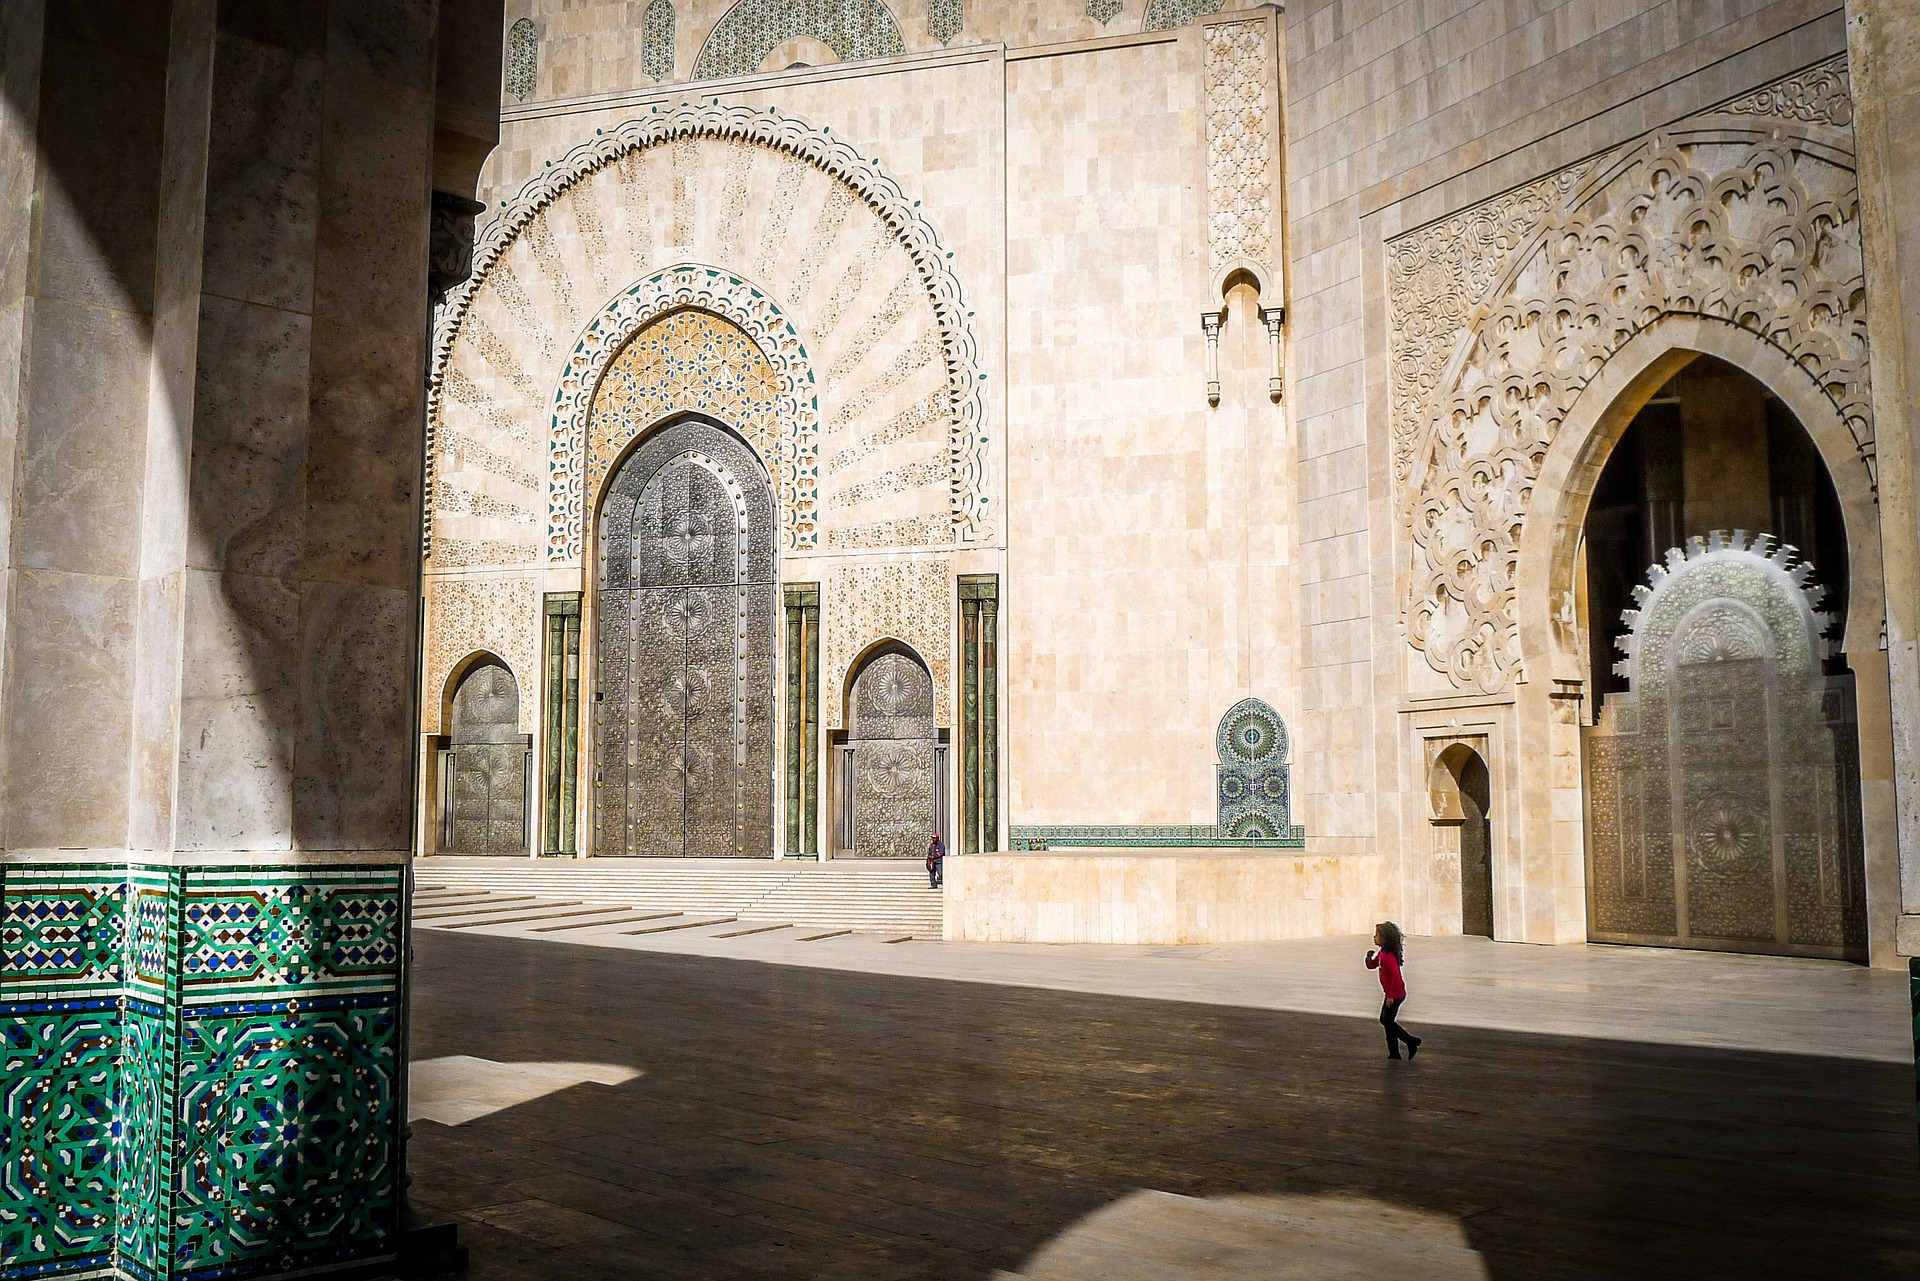
\includegraphics[width=0.5\columnwidth]
                                {contents/fig/mosque.jpg}
                \caption{caption示例}
            \end{figure}
        \end{texcodenoshad}
        \tcblower
        \begin{figure}[H]
            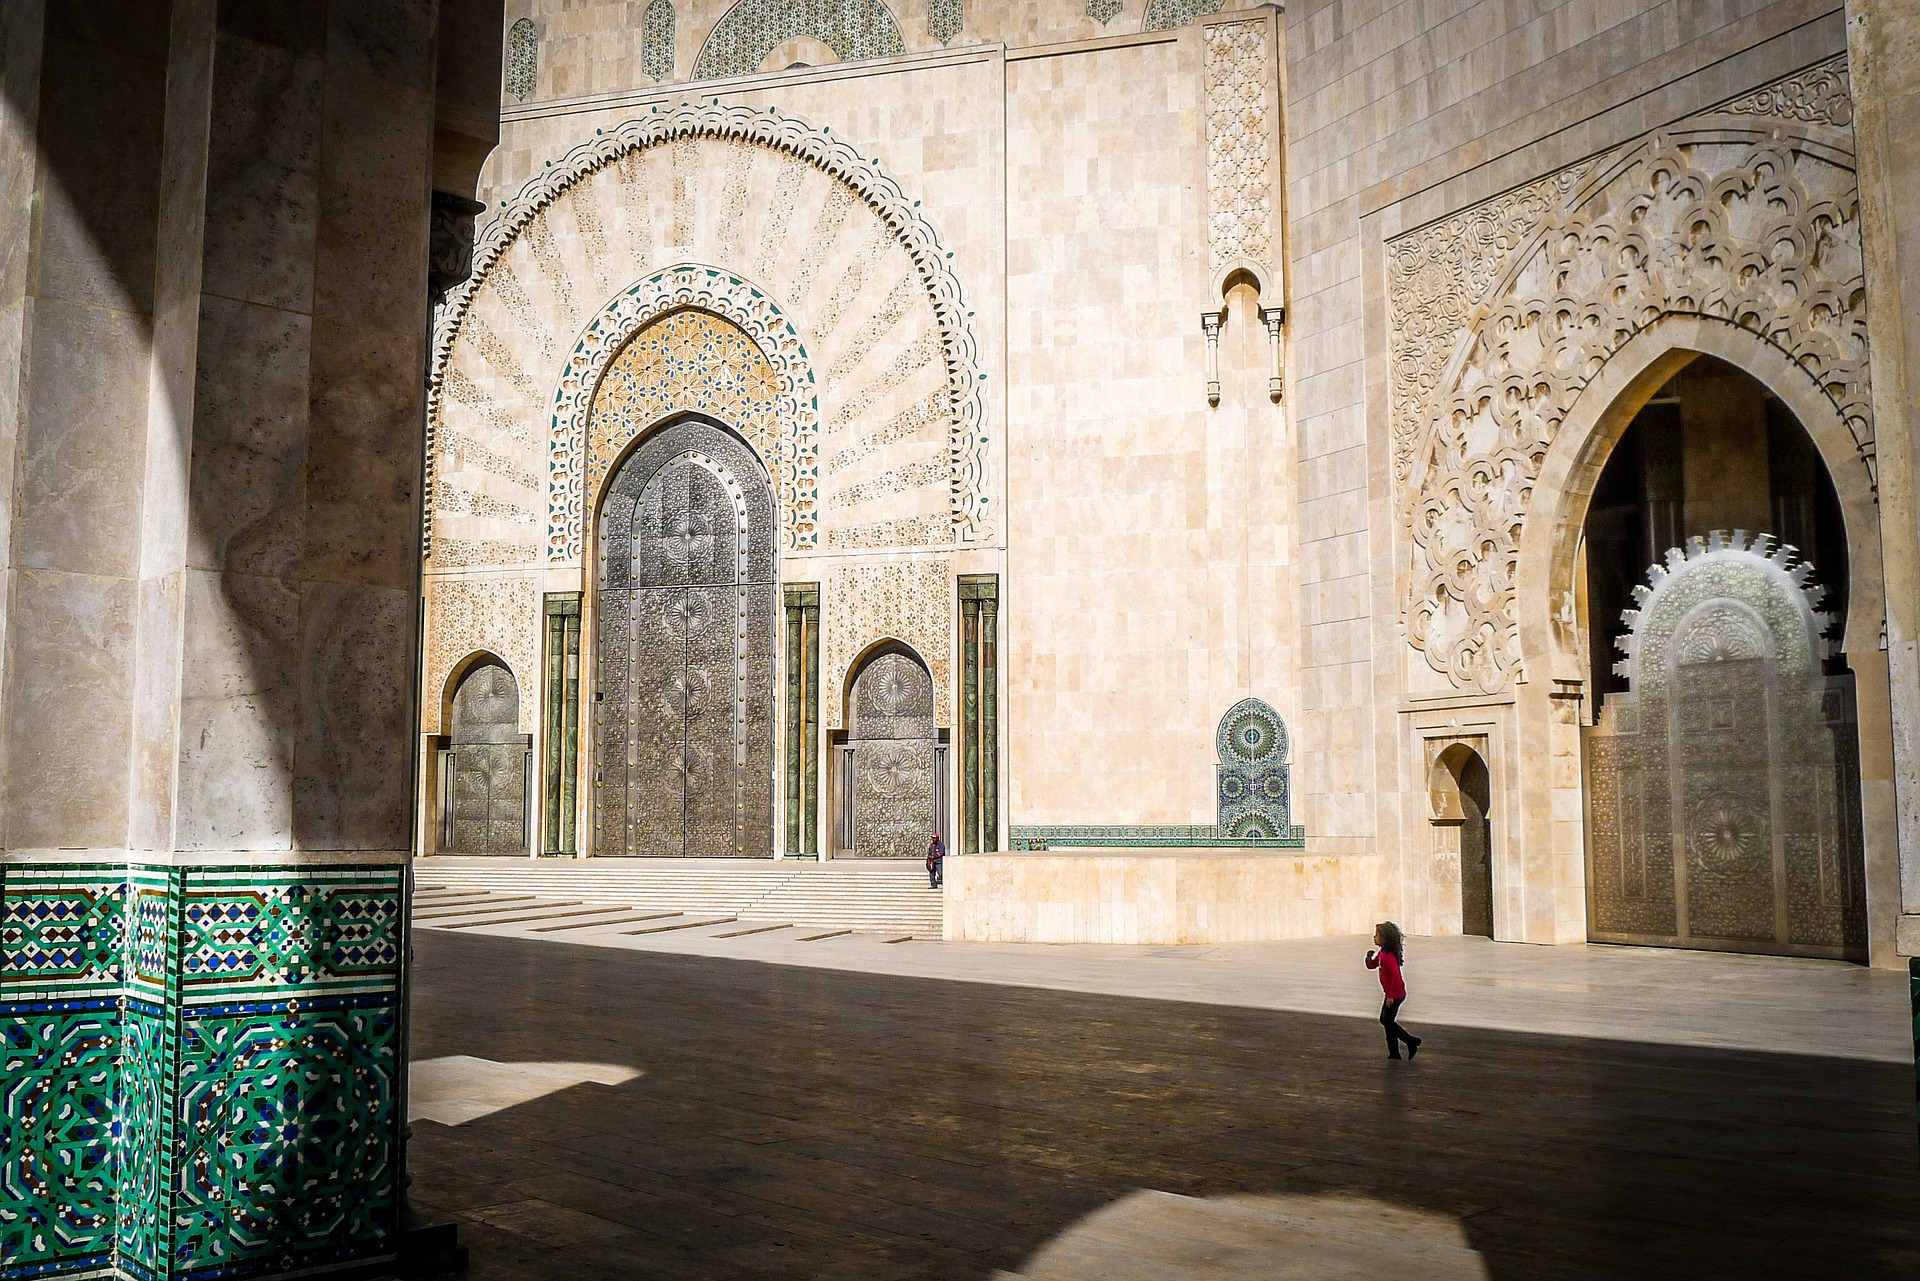
\includegraphics[width=0.5\columnwidth]
                            {contents/fig/mosque.jpg}
            \caption{caption示例}
        \end{figure}
    \end{texsepcode}
    如果要居中,则在Float环境中添加\highunderline{\textbackslash{}centering}即可(也可以在Float外或者Float内嵌套\highunderline{center}环境。)
    \begin{texsepcode}
        \begin{texcodenoshad}
            \begin{figure}[H]
                \centering
                \includegraphics[width=0.5\columnwidth]{contents/fig/mosque.jpg}
                \caption{居中示例}
            \end{figure}
        \end{texcodenoshad}
        \tcblower
        \begin{figure}[H]
            \centering
            \includegraphics[width=0.5\columnwidth]{contents/fig/mosque.jpg}
            \caption{居中示例}
        \end{figure}
    \end{texsepcode}
    \subsubsection{更改Float说明格式}
    默认中文下,\LaTeX{}会将表格编号为\textbf{表 n.},将图片编号为\textbf{图 n.},有时候我们可能有重新定制显示的需求,这实际上需要重新设置caption,具体如何设置请参考该宏包。

    % \todo{查看注释,又是个大的}
    % http://www.peteryu.ca/tutorials/publishing/latex_captions



    \subsection{Figure}\label{sub:figure}
    插入图片的基本使用可以参考\Ref{sec:graphics}一节,这里主要描述使用\highunderline{Figure}环境实现的各种图片的排版操作。

    \subsubsection{插入单张图片}
    在上一节已经有所演示,只需要用\highunderline{figure}环境包裹\highunderline{\textbackslash{}includegraphics}命令即可。
    
    \subsubsection{插入多个图片}
    插入多个图片可以直接在\highunderline{figure}环境中插入多个\highunderline{\textbackslash{}includegraphics}命令,但有时候需要对多个图片分别描述,因此需要使用\highunderline{subfigure}环境,如下:
    \begin{texshow}
        \begin{figure}[H]
            \subfigure[图片A]{ \label{subfig:show-a} % 标签永远都是可选项,需要引用的时候才需要添加
                \includegraphics[width=0.4\columnwidth]{mosque.jpg}
                \hspace{0.05\columnwidth} %声明水平间距,可以不添加,或者根据实际大小灵活更改
            }
            \subfigure[图片B]{
                \includegraphics[width=0.4\columnwidth]{mosque.jpg}
            }
            \caption{子图演示}
            \label{fig:sub-figure-show}
        \end{figure}
        % 如果需要居中,添加center环境或者使用\centering命令即可
    \end{texshow}
    
    % \todo{更改label/Tikz绘图/格式支持}
    % \subsubsection{插入环绕型图片}
    % \todo{环绕型图片}
    

    \subsubsection{列出图片目录}
    有时会有单独将所有的图片列出目录的需求,此时使用\highunderline{\textbackslash{}listoffigures}命令。
    
    \begin{quotation}
        一般是在文章目录后列出图片目录和表格目录。
    \end{quotation}
    
    % 如果需要手工插入图片目录,则使用
    
    
    \subsection{Table}\label{sub:table}
    
    \subsubsection{列出表格目录}
    有时会有单独将所有的表格列出目录的需求,此时使用\highunderline{\textbackslash{}listoftables}命令。
    
    \begin{quotation}
        一般是在文章目录后列出图片目录和表格目录。
    \end{quotation}